
\chapter{Descriptors}\label{descriptors}

\section{introduction}

Over the last decades, image feature detectors and descriptors have become popular tools in the computer vision community and they are being applied widely in a large number of applications. Image representation , image classification and retrieval  , object recognition and matching  3D scene reconstruction , motion tracking   texture classification , robot localization, all rely on the presence of stable and representative features in the image. Thus, detecting and extracting the image features are vital steps for these applications.
Hence The need for a Descriptor that can detect and extract Features 
and Since our HGR system needs a Features detector that can be stable in most cases which will  full fill our need to Recognize the Gesture performed by the user .


\textit{Note : The Definition of SIFT  Descriptor might be long and has a lot of Definitions because Sift is considered as the most  powerful and widely used local descriptor in object recognition and image classification Hence the Literature focus on it  , and as a guarantee  to ensure the understanding of  Sift definition and key words  we will summarize all Sift's  Definition  IN THE END OF EVERY SECTION }

\section{Definitions and Principles:}

\subsection{Global and Local Features}
the following definition was given by krig S in \cite{krig}. 
In the global feature representation, the image is represented by one multidimensional
feature vector, describing the information in the whole image.
In other words, the global representation method produces a single vector with values that
measure various aspects of the image such as color, texture or shape. Practically, a
single vector from each image is extracted and then two images can be compared by
comparing their feature vectors. For example, when one wants to distinguish images
of a sea (blue) and a forest (green), a global descriptor of color would produce quite
different vectors for each category. In this context, global features can be interpreted
as a particular property of image involving all pixels.
This property can be color histograms, texture, edges or even a specific descriptor extracted from some filters
applied to the image \cite{h}.\\ On the other hand, the main goal of local feature representation
is to distinctively represent the image based on some salient regions while
remaining invariant to viewpoint and illumination changes. Thus, the image is represented
based on its local structures by a set of local feature descriptors extracted
from a set of image regions called interest regions (i.e., keypoints) as illustrated in
Fig.\ref{fig:Ft1} Most local features represent texture within the image patch.

\begin{figure}[H]
\centering
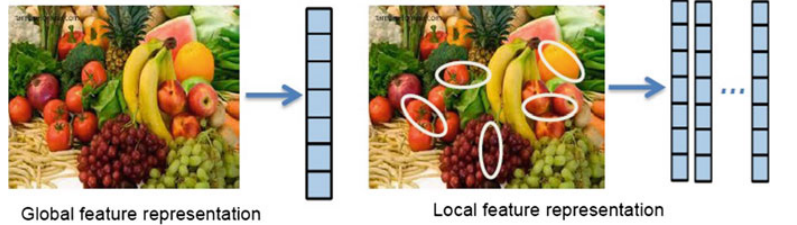
\includegraphics[width=0.9\textwidth]{img/features.PNG}
\caption{ Global and local image features representation }
\label{fig:Ft1}
\end{figure}

Generally, using what kind of features might greatly depend on the applications
on hand. Developers prefer the most discriminative ones. For example, a person with
a bigger nose and smaller eyes, and a person with a smaller nose and bigger eyes
may have similar mug shot in terms of histogram or intensity distribution. Then, local
features or the global pattern distilled from local feature clusters seem to be more
discriminative. Whereas, for very large datasets in the web scale image indexing
application, it is appropriate to consider global features. Also, global features are
useful in applications where a rough segmentation of the object of interest is available.
The advantages of global features are that they are much faster and compact
while easy to compute and generally require small amounts of memory.\\ Nevertheless,
the global representation suffers from well known limitations, in particular they
are not invariant to significant transformations and sensitive to clutter and occlusion.\\In some applications, such as copy detection, most of the illegal copies are very  similar to the original; they have only suffered from compression, scaling or limited
cropping. In contrast, the advantage of local features is their superior performance \cite{i}. Meanwhile, using local features for large scale image search have much higher performance than global features provide \cite{k}.\\ Besides, as the local structures are more distinctive and stable than other structures in smooth regions, it is expected to be more useful for image matching and object recognition.\\ However, they usually require a significant amount of memory because the image may have hundreds of local features.\\ As a solution for this problem, researchers suggest aggregating local image descriptors into a very compact vector representation and optimizing the
dimensionality reduction of these vectors \cite{k}


\subsection{Characteristics of Feature Detectors}

Tuytelaars and Mikolajczyk \cite{MM} define a local feature as \textit{ “it is an image pattern
which differs from its immediate neighborhood”.} Thus, they consider the purpose of
local invariant features is to provide a representation that allows to efficiently match
local structures between images. That is, we want to obtain a sparse set of local
measurements that capture the essence of the underlying input images and encode
their interesting structures. To meet this goal, the feature detectors and extractors
must have certain properties keeping in mind that the importance of these properties
depends on the actual application settings and compromises need to be made. The
following properties are important for utilizing a feature detector in computer vision
applications:
\begin{itemize}
\item Robustness, the feature detection algorithm should be able to detect the same feature
locations independent of scaling, rotation, shifting, photometric deformations,
compression artifacts, and noise
\item Repeatability, the feature detection algorithm should be able to detect the same
features of the same scene or object repeatedly under variety of viewing conditions.
\item Accuracy, the feature detection algorithm should accurately localize the image
features (same pixel locations), especially for image matching tasks, where precise
correspondences are needed to estimate the epipolar geometry.
\item Generality, the feature detection algorithm should be able to detect features that
can be used in different applications.
\item Efficiency, the feature detection algorithm should be able to detect features in new
images quickly to support real time applications.
\item Quantity, the feature detection algorithm should be able to detect all or most of the
features in the image. Where, the density of detected features should reflect the
information content of the image for providing a compact image representation.
\end{itemize}

\textbf{in this project We are going to use Local Features( descriptors) For its Efficiency and scale , Rotation  Invariant }\\
\section{Spectra descriptors :}
\subsection{SIFT - Scale Invariant Feature Transforms} \label{siftSection}

The Scale Invariant Feature Transform (SIFT) developed by Lowe \cite{lowe} is the most well known method for finding interest points and feature descriptors, providing invariance to scale, rotation, illumination, affine distortion, perspective and similarity
transforms, and noise. Lowe demonstrates that by using several SIFT descriptors together to describe an object, there is additional invariance to occlusion and clutter. We provide some detail here on SIFT since it is well designed and well known.


\begin{enumerate}
\item Scale-Space Extrema Detection :
The first stage of computation must search over all
scales and image locations, but it can be implemented efficiently by using a difference of-Gaussian
function to identify potential interest points that are invariant to scale and
orientation.
\item Keypoint localization :
At each candidate location, a detailed model is fit to determine
location, scale, and contrast. Keypoints are selected based on measures of their
stability.
\item Orientation assignment :
One or more orientations are assigned to each keypoint
location based on local image properties. All future operations are performed relative
to the assigned orientation, scale, and location for each feature, providing invariance
to these transformations.
\item Keypoint descriptor  :
The local image gradients are measured at the selected scale
in the region around each keypoint, and transformed into a representation that allows
for local shape distortion and change in illumination.
\end{enumerate}

An important aspect of this approach is that it generates large numbers of features that
densely cover the image over the full range of scales and locations.\\ A typical image of size
500$\times$500 pixels will give rise to about 2000 stable features (although this number depends
on both image content and choices for various parameters).\\ The quantity of features is
particularly important for object recognition, where the ability to detect small objects in
cluttered backgrounds requires that at least 3 to 6 features be correctly matched from each
object for reliable identification.
For image matching and recognition, features are first extracted from a set of reference
images and stored in a database.\\ A new image is matched by individually comparing
each feature from the new image to this previous database and finding candidate matching
features based on Euclidean distance of their feature vectors.\\
The keypoint descriptors are highly distinctive, which allows a single feature to find its
correct match with good probability in a large database of features. 



\subsection{Scale-Space Extrema Detection :}
As described in [\ref{siftSection}], we will detect keypoints using a sequential filtering approach
that uses efficient algorithms to identify candidate locations that are then examined
in further detail.\\ The first stage of keypoint detection is to identify locations and scales that
can be repeatably assigned under differing views of the same object. Detecting locations
that are invariant to scale change of the image requires that we search for stable features
across all possible changes of scale, using a continuous function of scale known as scale
space (Witkin, 1983).\\
It has been shown by Koenderink (1984) and Lindeberg (1994) that under a variety of reasonable assumptions the only possible scale space kernel is the Gaussian function.
Therefore, the scale space of an image is defined as a function, L(x, y, $\sigma$), that is produced
from the convolution of a variable scale Gaussian, G(x, y,$\sigma$), with an input image, I(x, y):\\

L(x, y, $\sigma$) = G(x, y,$\sigma$) * I(x, y),


where * is the convolution operation in x and y, and

\begin{align*} 
 G(x, y,\sigma )  =\frac{1}{2\pi\sigma^2} e^\frac{-( x^2 -  y^2)}{2\sigma^2}  
\end{align*}

To efficiently detect stable keypoint locations in scale space, we have proposed (Lowe,
1999) using scale space peaks in the difference-of-Gaussian function convolved with the
image, D(x, y, $\sigma$), which can be computed from the difference of two nearby scales separated
by a constant factor k:
\begin{align}
D(x, y, \sigma) &= (G(x, y, k\sigma) - G(x, y,\sigma) * I(x, y)\\
                 &= L(x, y, k\sigma) - L(x, y, \sigma) .
   \end{align}               
                  
There are a number of reasons for choosing this function. First, it is a particularly
efficient function to compute, as the smoothed images, L  need to be computed in any
case for scale space feature description, and D can therefore be computed by simple image
subtraction.

\begin{figure}[H]
\centering
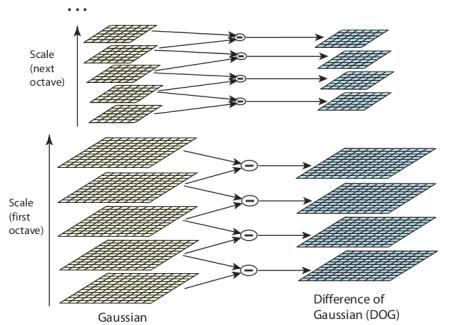
\includegraphics[width=0.8\textwidth]{img/sift_dog.jpg}
\caption{ DOG Principal .}
\label{fig:sift1}
\end{figure}

In addition, the difference-of-Gaussian function provides a close approximation to the
scale normalized Laplacian of Gaussian, $\sigma^2\nabla^2 G $
, as studied by Lindeberg (1994).\\Lindeberg
showed that the normalization of the Laplacian with the factor $\sigma^2$
is required for true scale invariance. In detailed experimental comparisons, Mikolajczyk (2002) found that the maxima and minima of $\sigma^2\nabla^2 G $  produce the most stable image features compared to a range
of other possible image functions, such as the gradient, Hessian, or Harris corner function.\\
The relationship between D and $\sigma^2\nabla^2G $
G can be understood from the heat diffusion
equation (parameterized in terms of $\sigma$ rather than the more usual t = $\sigma^2$):\\

\begin{align}
    \frac {\partial G} {\partial \sigma} = \sigma \nabla^2 G 
\end{align}




From this, we see that$\nabla^2$ G can be computed from the finite difference approximation to  $\frac{\partial G}{\partial \sigma }$ , using the difference of nearby scales at k$\sigma$ and $\sigma$ :\\


\begin{align}
      \sigma \nabla^2 G =   \frac {\partial G} {\partial \sigma} \approx   \frac {G(x,y,k \sigma) -  G(x,y,\sigma)}{ k \sigma - \sigma}  
\end{align}


and therefore,


\begin{align}
      G(x,y,k \sigma) -  G(x,y,\sigma)  \approx (k - 1)  \sigma^2\nabla^2G 
\end{align}

\begin{figure}[H]
\centering
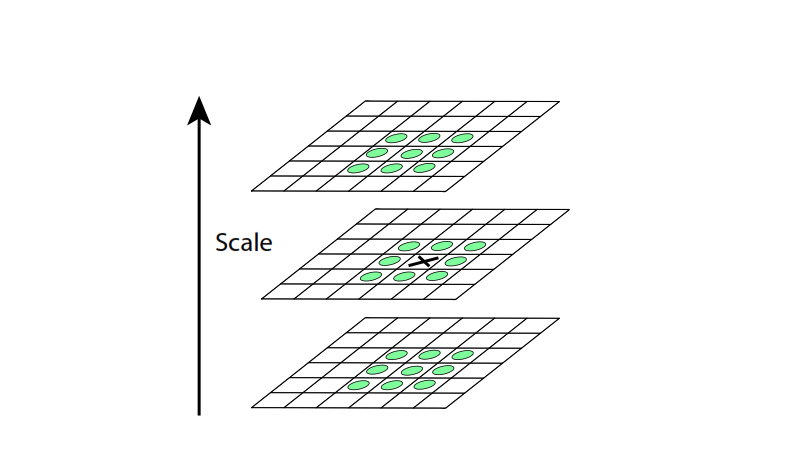
\includegraphics[width=1.0\textwidth]{img/sift2.PNG}
\caption{ Detection of maxima and minima of the difference-of-Gaussian .}
\label{fig:sift2}
\end{figure}

This shows that when the difference-of-Gaussian function has scales differing by a constant
factor it already incorporates the  $\sigma ^2 $
scale normalization required for the Laplacian. \\The
factor (k-1) in the equation is a constant over all scales and therefore does not influence
peak location. The approximation error will go to zero as k goes 1, but in practice we have
found that the approximation has almost no impact on the stability of peak detection or
localization for even significant differences in scale, such as $k= \sqrt{2}$
An efficient approach to construction of D(x; y;$\sigma$) is shown in Figure \ref{fig:sift1}. The input image
is incrementally convolved with Gaussians to produce images separated by a constant
factor k in scale space, shown stacked in the left column. \\We choose to divide each octave
of scale space (i.e., doubling of $\sigma$) into an integer number, s, of intervals, so $k = 2^{1/\mathbf{s}}$
Adjacent image scales are subtracted to produce the difference-of-Gaussian images shown
on the right. Once a complete octave has been processed, we resample the Gaussian image
that has twice the initial value of $\sigma$ by taking every second pixel in each row and column. \newline

The accuracy of sampling relative to $\sigma$ is no different than for the previous octave, while
computation is greatly reduced.

\textbf{Summary of the section :}

In the first step of SIFT, it generates several octaves of the original image. Each octave's image size is half the previous one. Within an octave, images are progressively blurred using the Gaussian Blur operator.
next we use all these octaves to generate Difference of Gaussian images ( Dog ) Two consecutive images in an octave are picked and one is subtracted from the other. Then the next consecutive pair is taken, and the process repeats. This is done for all octaves. The resulting images are an approximation of scale invariant laplacian of gaussian which is good for detecting keypoints .


\subsection{Keypoint localization :}
We wish to identify locations in image scale space that are
invariant with respect to image translation, scaling, and rotation,
and are minimally affected by noise and small distortions.\\
Lindeberg \cite{e} has shown that under some rather
general assumptions on scale invariance, the Gaussian kernel
and its derivatives are the only possible smoothing kernels
for scale space analysis.\\
To achieve rotation invariance and a high level of efficiency,
we have chosen to select key locations at maxima
and minima of a difference of Gaussian function applied in
scale space. This can be computed very efficiently by building
an image pyramid with resampling between each level.
Furthermore, it locates key points at regions and scales of
high variation, making these locations particularly stable for
characterizing the image.\\ Crowley and Parker \cite{f} and Lindeberg
\cite{e} have previously used the difference-of-Gaussian in
scale space for other purposes. In the following, we describe
a particularly efficient and stable method to detect and characterize
the maxima and minima of this function.\\
As the 2D Gaussian function is separable, its convolution
with the input image can be efficiently computed by applying
two passes of the 1D Gaussian function in the horizontal
and vertical directions:

\begin{align}
     g(x)  =\frac{1}{\sqrt{2\pi}\sigma} e^\frac{x^2}{2\sigma^2}
\end{align}


For key localization, all smoothing operations are done using
$\sigma = \sqrt{2}$ , which can be approximated with sufficient accuracy
using a 1D kernel with 7 sample points.\\
The input image is first convolved with the Gaussian
function using $\sigma = \sqrt{2}$ to give an image \textit{A}. This is then
repeated a second time with a further incremental smoothing
of $\sigma = \sqrt{2}$ to give a new image, \textit{B}, which now has an
effective smoothing of $\sigma$ =2. The difference of Gaussian
function is obtained by subtracting image B from A, resulting
in a ratio of $2/\sqrt{2}$ = $ \sqrt{2}$ between the two Gaussians.\\
To generate the next pyramid level, we resample the already smoothed image B using bilinear interpolation with a
pixel spacing of 1.5 in each direction.\\ While it may seem
more natural to resample with a relative scale of$\sqrt{2}$,the
only constraint is that sampling be frequent enough to detect
peaks.\\ The 1.5 spacing means that each newsample will
be a constant linear combination of 4 adjacent pixels. This
is efficient to compute and minimizes aliasing artifacts that
would arise from changing the resampling coefficients.\\
Maxima and minima of this scalespace function are determined
by comparing each pixel in the pyramid to its
neighbours. First, a pixel is compared to its 8 neighbours at
the same level of the pyramid.\\ If it is a maxima or minima
at this level, then the closest pixel location is calculated at
the next lowest level of the pyramid, taking account of the
1.5 times resampling. If the pixel remains higher (or lower)
than this closest pixel and its 8 neighbours, then the test is
repeated for the level above. Since most pixels will be eliminated
within a few comparisons, the cost of this detection is
small and much lower than that of building the pyramid.\\
If the first level of the pyramid is sampled at the same rate
as the input image, the highest spatial frequencies will be ignored.
This is due to the initial smoothing, which is needed
to provide separation of peaks for robust detection. Therefore,
we expand the input image by a factor of 2, using bilinear
interpolation, prior to building the pyramid. This gives
on the order of 1000 key points for a typical
512$\times$512 pixel
image, compared to only a quarter as many without the initial
expansion.

\textbf{Summary of this section :}

Here, we detected the maxima and minima in the DoG images generated in the previous step. This is done by comparing neighbouring pixels in the current scale, the scale "above" and the scale "below".


\subsection{Orientation assignment :}
By assigning a consistent orientation to each keypoint based on local image properties,
the keypoint descriptor can be represented relative to this orientation and therefore achieve
invariance to image rotation.\\ This approach contrasts with the orientation invariant descriptors
of Schmid and Mohr (1997), in which each image property is based on a rotationally
invariant measure.\\ The disadvantage of that approach is that it limits the descriptors that
can be used and discards image information by not requiring all measures to be based on a
consistent rotation.\\

Following experimentation with a number of approaches to assigning a local orientation,
the following approach was found to give the most stable results. The scale of the
keypoint is used to select the Gaussian smoothed image, L, with the closest scale, as all
computations must be performed in a scale invariant manner. For each image sample, $L_{x,y}$ ,the gradient magnitude, m, and orientation, $\theta$, is precomputed using pixel differences:

\begin{align}
 m  =\sqrt{(L_{x+1,y} - L_{x-1,y})^2 + (L_{x,y+1} - L_{x,y-1})^2}
\end{align}
\begin{align}
  \theta = \tan^{\small{-1}}\frac{(L_{x,y+1} - L_{x,y-1})}{(L_{x+1,y} - L_{x-1,y})}
\end{align}

An orientation histogram is formed from the gradient orientations at all sample points
within a circular window around the keypoint. Each sample added to the histogram is
weighted by its gradient magnitude and by a Gaussian-weighted circular window with a $\sigma$
three times that of the scale of the keypoint. The orientation histogram has 36 bins covering
the 360 degree range of orientations.
Peaks in the orientation histogram correspond to dominant directions of local gradients.
The highest local peak in the histogram is detected, and then any other local peak that is
within 80\% of the highest peak is used to also create a keypoint with that orientation.
Therefore, for locations with multiple peaks of similar magnitude, there will be multiple
keypoints created at the same location and scale but different orientations. Only about
15\% of points are assigned multiple orientations, but these contribute significantly to the
stability of matching. Finally, a parabola is fit to the 3 histogram values around each peak
to interpolate the peak position for better accuracy.


\textbf{summary of the section :}

To assign an orientation we use a histogram and a small region around it. Using the histogram, the most prominent gradient orientation(s) are identified. If there is only one peak, it is assigned to the keypoint. If there are multiple peaks above the 80\% mark, they are all converted into a new keypoint (with their respective orientations).

\subsection{Keypoint descriptor :}

Figure \ref{fig:sift4} illustrates the computation of the keypoint descriptor. First the image gradient
magnitudes and orientations are sampled around a keypoint, using the scale of the keypoint
to select the level of Gaussian blur for the image. For efficiency, the gradients are precomputed
for all levels of the pyramid as described in Section 4.1.3 . These are illustrated with
small arrows at each sample location on the left side of Figure \ref{fig:sift4}

\begin{figure}[H]
\centering
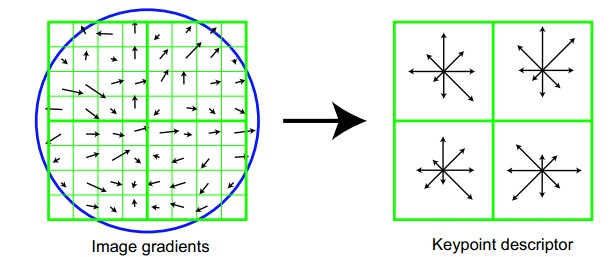
\includegraphics[width=0.8\textwidth]{img/sift4.jpg}
\caption{ Keypoint descriptor }
\label{fig:sift4}
\end{figure}

A Gaussian weighting function with $\sigma$ equal to one half the width of the descriptor
window is used to assign a weight to the magnitude of each sample point. This is illustrated
with a circular window on the left side of Figure \ref{fig:sift4}, although, of course, the weight falls off smoothly. The purpose of this Gaussian window is to avoid sudden changes in the
descriptor with small changes in the position of the window, and to give less emphasis
to gradients that are far from the center of the descriptor, as these are most affected by
misregistration errors.
The keypoint descriptor is shown on the right side of Figure \ref{fig:sift4}. It allows for significant
shift in gradient positions by creating orientation histograms over 4$\times$4 sample regions. The
figure shows eight directions for each orientation histogram, with the length of each arrow
corresponding to the magnitude of that histogram entry. A gradient sample on the left can
shift up to 4 sample positions while still contributing to the same histogram on the right,
thereby achieving the objective of allowing for wider local positional shifts.
It is important to avoid all boundary affects in which the descriptor abruptly changes as
a sample shifts smoothly from being within one histogram to another or from one orientation
to another. Therefore, linear interpolation is used to assign a weight to each histogram
entry according to the distance of the sample from its central value, and the gradient magnitude
of a sample is distributed into the histogram accumulators according to these weights.
The descriptor is formed from a vector containing the values of all the orientation histogram
entries, corresponding to the lengths of the arrows on the right side of Figure \ref{fig:sift4}. The
figure shows a 2$\times$2 array of orientation histograms, whereas our experiments below show
that best results are achieved with a 4$\times$4 array of histograms with 8 orientation bins in each.
Therefore, the experiments in this paper use a 4$\times$4$\times$8 = 128 element feature vector for each
keypoint.
Finally, the feature vector is normalized to reduce the effects of illumination change.
First, the vector is normalized to unit length. A change in image contrast in which each
pixel value is multiplied by a constant will multiply gradients by the same constant, so this
contrast change will be cancelled by vector normalization. A brightness change in which a
constant is added to each image pixel will not affect the gradient values, as they are computed
from pixel differences. However, non linear illumination changes can also occur due
to camera saturation or illumination changes that affect surfaces with different orientations
by differing amounts. These effects can cause a large change in relative magnitudes for
some gradients, but are less likely to affect the gradient orientations. Therefore, we reduce
the influence of gradient magnitudes by thresholding the values in the unit feature vector to
each be no larger than 0.2, and then renormalizing to unit length. This means that matching
the magnitudes for large gradients is no longer as important, and that the distribution of
orientations has greater emphasis. The value of 0.2 was determined experimentally using
differing illuminations for the same objects\\

\textbf{Summary of the section }

Sift take  a 16x16 window of "in-between" pixels around the keypoint. split that window into sixteen 4x4 windows. From each 4x4 window it generate a histogram of 8 bins. Each bin corresponding to 0-44 degrees, 45-89 degrees. Gradient orientations from the 4x4 are put into these bins. This is done for all 4x4 blocks. Finally, it normalize the 128 values .

\subsection{Speeded Up Robust Features (SURF) :} \label{surf}
SURF (Speeded Up Robust Features), is a feature detector, we talked about SIFT before, and SURF is sort of derivative of SIFT. SURF is based on sums of 2D Haar wavelet responses and makes an efficient use of integral images.

we will not go through  the whole literature  of SURF, because its idea is very similar to SIFT, so we will only talk about \textbf{the difference between these two methods}.

\subsection{ABOUT HESSIAN}
In Sift method, we use Difference of Gaussian (DoG) to build the image pyramid, and in Surf, we simply use an integer approximation to the determinant of Hessian blob detector .

Given a pixel, the Hessian of this pixel is something like:
$\sigma^2\nabla^2G$ \\

\begin{gather}
H(f(x,y)) =
\begin{bmatrix}
                 {\frac {\partial^2 f} {\partial x^2}} && { \frac {\partial^2 f} {\partial x.\partial y} }\\
                 {\frac  {\partial^2 f}{\partial x.\partial y}} && { \frac {\partial^2 f} {\partial y^2}}
\end{bmatrix}
\end{gather}

For adapt to any scale, we filtered the image by a Gaussian kernel, so given a point X = (x, y), the Hessian matrix H(x,$\sigma$) in x at scale $\sigma$ is defined as:
\begin{gather}
 \mathcal{H}(x,\sigma) =
\begin{bmatrix}
                 {L_{xx}(x,\sigma)}  && {L_{xy}(x,\sigma)} \\
                 {L_{xy}(x,\sigma)} && {L_{yy}(x,\sigma)}
\end{bmatrix}
\end{gather}
where ${L_{xx}(x,\sigma)}$ is the convolution of the Gaussian second order derivative with the image I in point x, and similarly for ${L_{xy}(x,\sigma)}$ and ${L_{yy}(x,\sigma)}$.\\
First convolution, then second order derivative, we now approximate these two processes with one single filter.\\


\begin{figure}[H]
\centering
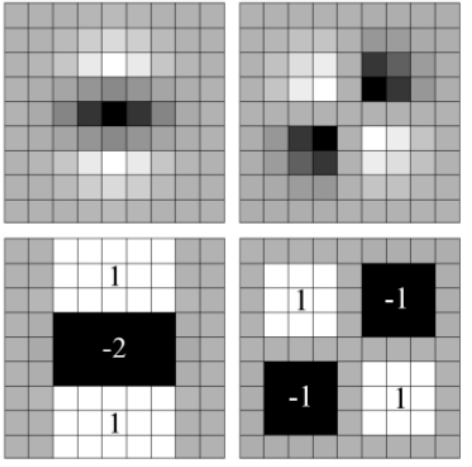
\includegraphics[width=0.55\textwidth]{img/surf4.PNG}
\caption{${L_{yy}(x,\sigma)}$ and${L_{xy}(x,\sigma)}$ Discretized
Gaussians and the approximations $D_{yy}$ and $D_{xy}$}
\label{fig:surf1}
\end{figure}

These approximate second order Gaussian derivatives and can be evaluated at a very low computational cost using integral images, and this is part of the reason why SURF is fast.

Now we can represent the determinant of the Hessian (approximated) as:

\begin{figure}[H]
\centering
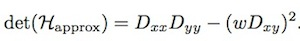
\includegraphics[width= 0.4\textwidth]{img/det.jpeg}

\label{fig:surfdet}
\end{figure}
and we can use 0.9 for w by Bay’s suggestion.

\subsection{ABOUT PYRAMID :}

In Sift, we use DOG to build image pyramids, the pyramid have several octaves, and there are several images layers in each octave. The difference between Sift pyramid and Surf pyramid is, in Sift, we use different scales of image; and in Surf, we use different scales of Gaussian masks, while the scale of image is always unaltered. By this, we save a lot of time by not downsampling image.

\begin{figure}[H]
\centering
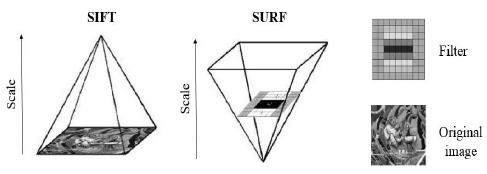
\includegraphics[width=0.6\textwidth]{img/surf2.png}
\caption{Where SIFT(left) downscales the image,
SURF(right) uses larger and larger filters}
\label{fig:surf2}
\end{figure}

 Instead of iteratively reducing the image size (left), the use of integral images allows the upscaling of the filter at constant cost (right).\\
 
 \subsection{ABOUT FEATURE DESCRIPTOR}
 In Sift, we use an orientation histogram, and find the largest orientation value and also those values that are over 80\% of the largest, and use these orientations as the main orientation of the feature descriptor. In Surf, we use the sum of the Haar wavelet response around the point of interest.

\begin{figure}[H]
\centering
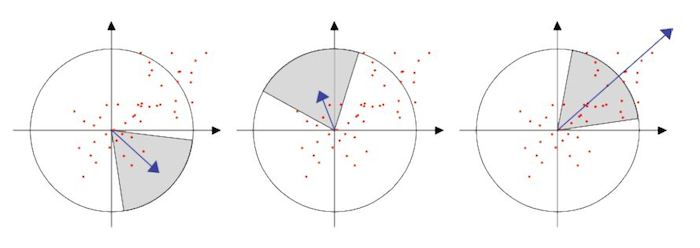
\includegraphics[width=0.6\textwidth]{img/surf3.jpg}
\caption{descriptor computation }
\label{fig:surf3}
\end{figure}

We first calculate the Haar wavelet responses in x and y direction within a circular neighborhood of radius 6s around the interest point, with s the scale at which the interest point was detected. We calculate the sum of vertical and horizontal wavelet responses in a scanning aria, then change the scanning orientation (add $\pi$/3), and recalculate, until we find the orientation with largest sum value, this orientation is the main orientation of feature descriptor.

Now it’s time to extract the descriptor. First we construct a square region centered around the feature point, and oriented along the main orientation we already got above, the size of this window is 20s,s is the scale at which the interest point was detected. Second we split this region up regularly into smaller 4$\times$4 square subregions, for each subregion, we compute Haar wavelet responses at 5$\times$5 regularly spaced sample points.


\begin{figure}[H]
\centering
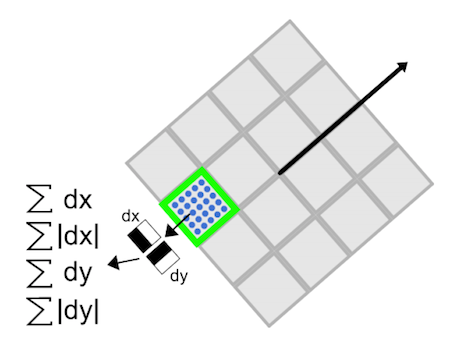
\includegraphics[width=0.5\textwidth]{img/surf5.png}
\caption{computation of dx and dy of Haar  }
\label{fig:surf5}
\end{figure}

We extract the sum of values of the responses in both x and y orientation, furthermore, we extract the sum of the absolute values of the responses, hence, each subregion has a 4-D descriptor vector v. Concatenating this for all 4$\times$4 subregions, our final descriptor is a 64-D vector. (In Sift, our descriptor is 128-D vector, so this is part of the reason that SURF is faster than Sift.)\\


\section{Differences and Preference :}
The two main advantages of SURF over SIFT is that SURF uses Laplacian of Gaussian so as to have a distinction
between background and foreground features, and secondly, SURF uses only 64 dimensional vector compared to 128 dimensional vector for SIFT . This helps in fast feature computation and also the quick matching capability.
The two different steps used by SURF to determine the local descriptor vectors are A. Keypoint Detection B. Keypoint Descriptor, which were  explained above \ref{surf} and \ref{siftSection}.

This makes Surf as our best candidate for gesture recognition  since it offers high number of stable features against Scale invariance and rotation invariance , of course lesser than Sift but it does not worth the Computational operations of up scaling pyramid used in sift Nor the \textbf{valuable }time consumed .

later on we will Experimentally demonstrate that Surf achieved  better accuracy than sift in Hand gesture Recognition  . However Even if Surf is less expensive than sift but still computationally expensive which is bad for our purposes ,Since what describe a Good HGR is its ability to interpret  and interact with the Signer performer in real time , That's where Fouriere descriptor Appears to give accurate and a Very Fast feature extractor which will meet our requirement for a robust and Real time application  .


\section{Fourier Shape Descriptor } \label{FDT}
The Fourier transformed coefficients from the Fourier
Descriptors of the shape represent the shape of the object in
the frequency domain. The general features of the shape can
be found in the lower frequency descriptors, while the higher
frequency descriptors contain information about the shape
details \cite{20}
Before applying Fourier transform on the shape boundary, it
is first normalized for matching purposes; this is done by
sampling the boundary of each shape to have the same number
of data points. The larger the number of sampled points the
more details in the representation of the shape this results in
more accurate matching. While a smaller number of sampled
points reduce the accuracy of the matching results but on the
other hand it will improve the computational efficiency. \\

After normalization we to apply Fourier transform to the
shape signature. A shape signature is any 1-D function
representing 2-D areas or boundaries. The shape signature we
used is complex coordinates. A complex coordinates function
is the complex form of the boundary coordinates \cite{20}. \\
\begin{gather}
    z_{i} = x_{i}+j y_{i} , i\in [1,N]
\end{gather}\\
For each shape we select N points with equal point
sampling. In order to facilitate the use of Fast Fourier
Transform (FFT), the number of sampled points is chosen to
be power of two. Assuming the number of sampled points is
N the Fourier transform gives N Fourier coefficients Cl. The
coefficients are usually called Fourier descriptors of the shape. 
\begin{gather}
C_{l}= \sum_{i=0}^{N-1} z_{i}e{\frac{-j 2\pi il}{N}} , l = 0,...,N-1
\end{gather}
The magnitude of the Fourier
Transform of this set forms a unique shape signature, which can be used for generalized
gesture classification.
In addition, this descriptor is rotationally invariant. Shifts in the silhouette contour
points, which is the cause of rotation, will be appear as phase delays in frequency
domain. However, since only the magnitude of the Fourier coefficients is considered,
the phase (or equivalently, the rotation) is ignored. So, this method is rotationally
invariant while remaining computationally fast\\


\textbf{Generating the Fourier Descriptor: }
\begin{enumerate}
    \item $X_{c} = \frac{1}{N}\sum_{n=0}^{N-1} x(i) , Y_{c} = \frac{1}{N}\sum_{n=0}^{N-1} y(i)  = 1$ , where N is number of hand object pixels 
    \item Take the magnitude of the N point DFT of these points :\\
              \textbf{ abs(FT{r[n]}) = a[m] , for m = 0..N-1 }.
    \item Normalize the Fourier coefficients by the DC value (Scale Invariance) .
    \item Keep the first 7 normalized coefficients (skip DC, which is always 1) .

\end{enumerate}


This is the Fourier Descriptor for a single shape.\\

\textbf{Make a Dictionary : } For a set of images of the same gesture, compute the average Fourier shape descriptor and add it to the dictionary with the same label.  Repeat for all desired gestures.

\textbf{Classification  : }Compute the Fourier descriptor for each new sample.  Compare it with each stored gesture in the dictionary using  Euclidean distance measure.  The label of the minimum distance is the desired gesture( Nearest Neighbor happens to be the most efficient method of classification )

\subsection{Covariance Matrix Approach :}
This approach \cite{21}
performs human action recognition by looking at a sequence of whole body silhouettes
over time, a silhouette tunnel, captured by the Kinect. A 13 dimensional feature vector
is defined, where 3 values are row, column, and time, 8 values are based on the shape of
the silhouette, and the last 2 are a measure of the temporal similarity.
However, this feature vector is general enough to work with hand silhouettes in addition
to full bodies. So, it is possible to modify the shape feature vector to work with static
hand gestures by reducing the dimensionality. This can be accomplished by removing
the time dependence and temporal similarity terms. The result is a generalized 10
dimensional feature vector applicable to static shape recognition.\\

\textbf{Create the Feature Vector :}\\
\begin{enumerate}
    \item Compute the 10-dimensional feature vector adapted from Guo \cite{21} : 
    
    \item f(x,y) = [x,y,de,dw,dn,ds,dne,dse,dnw]
    \begin{itemize}
        \item x = col , y=row
        \item d =  Euclidean distance from (x,y) to the nearest boundary point in the specified
direction \\
east, west, north, south, northeast, southwest, southeast, northwest
    \end{itemize}
    \item Scale Invariance 
    \begin{itemize}
        \item Divide each spatial feature by the square root of the silhouette area
     
    \end{itemize}
    \item Compute the Covariance Matrix: 
    \begin{itemize}
        \item $cov(f(\textbf{S}))=\frac{1}{|S|}\sum_{(x,y) \in S }(f(x,y)-\mu_{F})(f(x,y)-\mu_{F})^{T}$
        \item \textbf{S} = area of silhouettte 
        \item $\mu_{F} = \frac{1}{|S|}\sum_{(x,y) \in S } f(x,y) $
    \end{itemize}
    
\end{enumerate}
\textbf{Build a Dictionary }\\
For a set of images of the same gesture, compute the Covariance Matrix and add it to
the dictionary with the same label. Repeat for all desired gestures.\\
\textbf{Classification }\\
As noted in Guo \cite{21}, the set of all covariance matrices lie on a Riemannian
manifold. So, a Euclidean distance measure cannot be used. Instead, the distance
between two covariance matrices on this manifold is defined as:\\
$$d(C,C') = \sqrt{\sum_{k=1}^{10} (\ln \lambda_{k}(C,C'))^{2}}$$ \\
\texttt{where $\lambda_{k}(C,C')$ are generalized eigenvalues of C and C'\\
C = convariance Matrix of new sample ,  C' = Reference from dictionary  } \\

The label of the minimum distance gesture is used for classification .

\begin{table}[!h]
\centering
\caption{Pros and Con of Covariance approach }
\label{my-label}
\begin{tabular}{lllll}
\cline{1-2}
\multicolumn{1}{|l|}{\textbf{\begin{tabular}[c]{@{}l@{}}Pros:\\  1. Complex Gesture .\\  2. High accuracy.\\  3. Scale invariant.\end{tabular}}} & \multicolumn{1}{l|}{\textbf{\begin{tabular}[c]{@{}l@{}}Con :\\ 1. Not rotation Invariant . \\           \\        \\ \end{tabular}}} &  &  &  \\ \cline{1-2}
                                                                                                                                                 &                                                                                                           &  &  &  \\
                                                                                                                                                 &                                                                                                           &  &  &  \\
                                                                                                                                                 &                                                                                                           &  &  & 
\end{tabular}
\end{table}

\newpage
 
 \section{ Conclusion : }
 in this chapter we went through Two types of descriptors :
 
\textbf{the first} are  Local descriptors SIFT and SURF  descriptors that typically involves more intense computations and algorithms, often requiring floating point
calculations, and may consume considerable memory.but generally they give a high  accuracy Additionally to their stable performance even against scale variation and Rotation variation too , the following table is summarizing the Differences of these two descriptors :

\begin{table}[!h]
\centering
\caption{COMPARISON OF SIFT AND SURF}
\label{surfvssift}
\begin{tabular}{l|l|l|ll}
\cline{2-3}
\textbf{}                                                                                     & \textbf{SIFT}                                                                                                                                                     & \textbf{SURF}                                                                                                                             &  &  \\ \cline{1-3}
\multicolumn{1}{|l|}{\textbf{\begin{tabular}[c]{@{}l@{}}Keypoint\\ Detection\end{tabular}}}   & \textbf{\begin{tabular}[c]{@{}l@{}}Different scale image\\ convoluted with\\ Gaussian function\end{tabular}}                                                      & \textbf{\begin{tabular}[c]{@{}l@{}}Original Image is\\ convoluted with\\ Different scale box\\ filter\end{tabular}}                       &  &  \\ \cline{1-3}
\multicolumn{1}{|l|}{\textbf{\begin{tabular}[c]{@{}l@{}}Keypoint\\ Description\end{tabular}}} & \textbf{\begin{tabular}[c]{@{}l@{}}Gradient amplitude of\\ a square area is\\ calculated with\\ maximum gradient\\ strength as the main\\ direction\end{tabular}} & \textbf{\begin{tabular}[c]{@{}l@{}}A Haar Wavelet response\\  is used to\\ calculate \\ each sector in\\ a \\ circular area\end{tabular}} &  &  \\ \cline{1-3}
\multicolumn{1}{|l|}{\textbf{Dimensions}}                                                     & 128                                                                                                                                                               & 64                                                                                                                                        &  &  \\ \cline{1-3}
\end{tabular}
\end{table}



\textbf{The second } are Basis Space descriptors   , A basis space is composed of a set of functions, the basis functions, which are
composed together as a set, such as a series like the Fourier series and covariance Matrix  . 

Fourier descriptors represent feature data as sine and cosine terms, which can be
observed in a Fourier Power Spectrum. The Fourier series, Fourier transform, and Fast
Fourier transform are used for a wide range of signal analysis, including 1D, 2D, and 3D
problems. No discussion of image processing or computer vision is complete without
Fourier methods .

With this summary we are done from Feature detection / extraction and we will move on to the next Phase of building  our HGR System , which is  Feature classification using Machine learning algorithms that's going to be the goal of next section .